\chapter{Data collection}

%TOMATOES SYNTH + WOOD

\section{Data}
\label{sec_data}

Three sets of data were used in the numerical experiments.
The first are the synthetic ellipsoids generated with a naive straightforward method, see subsection \ref{subsec_ray_data}.
The second are the data generated with the ray emulation approach, see subsection \ref{subsec_naive_data}.
Finally, the third is the real data recorded with Intel RealSense D435i camera, see subsection \ref{subsec_real_data}.
Let us describe these sets of data.

\subsection{Naive synthetic ellipsoids generation}
\label{subsec_naive_data}

The first dataset contains points evenly distributed on the surface of ideal ellipsoids.
The ellipsoid is described by its center, semiaxes, and rotation.
After specifying those, a point cloud is created, consisting of points on the surface of the ellipsoid.
These data were used as the simplest possible to evaluate the algorithm's performance.
As one might expect, the error on clear data was precisely zero, so data with additive normal noise was considered as well, see Table \ref{tabularx:iou_tables} and Table \ref{tab:vol_table}.

The point clouds that are generated this way are different from the real ones due to the non-uniform surface coverage in the real data and only partial visibility to the real camera.

\subsection{Ray emulation-based synthetic data generation}
\label{subsec_ray_data}

Thus, an alternative approach was taken with a proper geometrical model of the camera.
Stereoscopic vision, either active or passive, relies on the difference in the appearance of the same objects from two distinct viewpoints.
Their correspondence allows for the reconstruction of the depth in the scene.
It should be noted that with such an approach the ellipsoid is covered with points not uniformly, see Figure \ref{fig_tomatoes_projection}.
An explicit geometrical model was used to obtain data that closely resembles the real point clouds.

\label{ell_line_int}
According to the used model, a tomato can be represented as an ellipsoid. 
Hence, the point cloud obtained from a real tomato can be approximated as the point cloud of an ideal ellipsoid. 
In this section, the process of image formation is considered.

\begin{figure}[!htb]
  \centering
  %\begin{subfigure}{0.48\textwidth}
  %    \centering
      \includegraphics[width=0.8\textwidth]{images/tomato.png}
      \caption{Scheme of the ray tracing-based approach to point cloud generation. On the left the focal point of the camera is presented, the red grid in the middle is the camera matrix, and the rays casted from through it intersect with the surface of the ellipsoid in the points marked with cyan triangles.}
      \label{fig_tomatoes_projection}
  %\end{subfigure}
\end{figure}

The leftmost violet point in Figure \ref{fig_tomatoes_projection} represents the focal center of the camera, while the red points correspond to the light-sensitive pixels of the camera matrix. 
A line between the blue and red points visualizes a beam of light reflected from the ellipsoid that intersects with the camera matrix.
Extending this line to intersect with the ellipsoid yields a point in the point cloud (cyan triangles). 
%To create a more realistic point cloud, it is essential to introduce noise; however, for the purposes of this discussion, we will first consider the ideal scenario. 
Thus, the problem of finding the intersection of a line formed by two points with the ellipsoid needs to be addressed.

Let us consider an ellipsoid defined by $S$ (scale matrix), $R$ (rotation matrix), and $t$ (translation vector), along with a line formed by points $A$ and $B$.

First, let us transform the ellipsoid so that it becomes a unit sphere at the origin in order to simplify the problem.
The points $A$ and $B$ will be transformed as follows:

\begin{align*}
A' &= S^{-1} R^T (A - t), \\
B' &= S^{-1} R^T (B - t).
\tag{19}
\end{align*}

The direction vector defining the light beam line in the new coordinates can be found as:

\begin{align*}
a &= \frac{A' - B'}{\|A' - B'\|}.
\tag{20}
\end{align*}

The solution for the line-sphere intersection yields two points $P_1$ and $P_2$, that can be found according to the subsequent computational steps derived from solving a quadratic equation, if $\Delta \geq 0$.

\begin{align*}
\Delta & = (a^T A')^2 - (A')^T A  + 1, \\
C' & = A' - a^T A' a, \\
P_1' & = C' - a \sqrt{\Delta}, \\
P_2' & = C' + a \sqrt{\Delta}, \\
P_1 & =  R S (P_1' + t), \\
P_2 & =  R S (P_2' + t). \\
\tag{21}
\end{align*}

By repeating this algorithm for each red point representing pixels, an array of points that lie on the ellipsoid is formed, see Figure \ref{fig:synth_segment_clean}.
After that the noise is added into the data, see Figure \ref{fig:synth_segment_noise}.
The amplitude of noise was chosen in accordance with the real data.

\begin{figure}
  \centering

  \begin{subfigure}[b]{0.42\textwidth}
      \centering
      \includegraphics[width=\textwidth]{images/segment_image_without_noise.png}
      \caption{Example of a point cloud of an ellipsoid segment without noise}
      \label{fig:synth_segment_clean}
  \end{subfigure}
  \hfill
  \begin{subfigure}[b]{0.42\textwidth}
      \centering
      \includegraphics[width=\textwidth]{images/segment_image_with_noise.png}
      \caption{Example of a point cloud of an ellipsoid segment with noise}
      \label{fig:synth_segment_noise}
  \end{subfigure}
  \caption{Samples from a part of the synthetic dataset, generated with the ray tracing: (a) clear (b) with additive normal noise.}
  %\label{fig_segments}
\end{figure}

\subsection{Real data}
\label{subsec_real_data}

%\subsubsection{Tomatoes on a horizontal plane}\label{sec:ch3/sec3/subsec2/subsubsec1}

\begin{figure}[!htb]
  \centering
  %\begin{subfigure}{0.48\textwidth}
  %    \centering
      \includegraphics[width=0.8\textwidth]{images/wood_data.png}
      \caption{Sample point cloud from the real part of the dataset. Tomatoes and a rubber ball are placed on a wooden support.}
      \label{fig:wood_data}
  %\end{subfigure}
\end{figure}

The point cloud in the Figure \ref{fig:wood_data} is from the real part of the dataset.
These point clouds are a challenging piece of data.
Tomatoes are described by an ellipsoid model only in a certain approximation, varying from fruit to fruit and from strain to strain.
It means that even the best possible fit will result in a certain non-zero error.

Moreover, the real noise cannot be approximated by the normal noise model.
In the Figure \ref{fig:hist_for_segment_distances} the distribution of the algebraic distance from the ellipsoid surface is presented for the synthetic data.
In the Figure \ref{fig:wood_rs_55_pcds_distances_over_real_hist_plot_wood} the same is given for the real data.
It could be seen that the distribution for the real data is not unimodal and skewed for all three tomatoes considered, meaning that the real data does not fully comply with the used model.

The last considerable obstacle are the distortions that occur on the surface of the tomatoes.
The exact reasons behind this effect are not clear, but such a distorted appearance was noticed a number of times.

%\blue{
The ways to deal with these complications include the following.
In order to account for the tomatoes being not precisely ellipsoid a more general model of the fruit can be used, such as hyperellipsoids or even the most general case, such as a combination of shperical harmonics.
The noise with the complex distributions can be dealt with by standard RANCAS, as numerical experiments on the real data suggest.
Finally, end-to-end algorithms, such as neural networks, can be used.
%}

To test the algorithm on real data, a series of experiments was conducted with tomatoes located on a horizontal wooden board.
The experiment involved six tomatoes and one rubber ball, that were placed at a distance of between 10 and 15 \si{cm} from each other, see Figure \ref{fig:wood_data}.
The camera captured scenes at various angles of the board: 55, 60, 70, 80 and 90 degrees.
This made it possible to study the effect of the viewing angle on the perception of the shape of objects by the depth camera.
For each angle, 146 point clouds were taken.
Each point cloud contains approximately 111,000 points, where nearly 2,200 belong to the tomatoes.
For a single object this number varies from 831 points for the nearest one to 130 for the farthest.
The volume of the tomatoes ranges from 90 to 207 cubic \si{cm}.
For each tomato the ball their actual size and volume were measured, and the exact location relative to the camera was determined.
In this experiment, tomatoes were modeled as ideal spheres, where the radius of the sphere was determined by the average value of the semi-axes of the ellipsoid.
The tomatoes used were reasonably close to a sphere, which made it possible to make this assumption fair.
As a result, a dataset was created containing the centers and radii of objects, that were compared with the output of the algorithm.

\begin{figure}[!htb]
  \centering
      \includegraphics[width=0.8\textwidth]{images/wood_synth_distances_over_real_hist_plot_wood.pdf}
      \caption{Distribution of the algebraic distance between the points and the surface of the best fitted ellipsoid model for synthetic data. A clear unimodal distribution can be seen.}
      \label{fig:hist_for_segment_distances}
\end{figure}

\begin{figure}[!htb]
  \centering
  %\begin{subfigure}{0.48\textwidth}
  %    \centering
      \includegraphics[width=0.8\textwidth]{images/wood_rs-55_pcds_distances_over_real_hist_plot_wood2}
      \caption{Distribution of the algebraic distance between the points and the surface of the best fitted ellipsoid model for three tomatoes from the real data. For all three of them the distribution is rather noisy and clearly not unimodal, suggesting that the real data is significantly more challenging than synthetic.}
      \label{fig:wood_rs_55_pcds_distances_over_real_hist_plot_wood}
  %\end{subfigure}
\end{figure}

The real data was captured with Intel RealSense D435i.
The exposure and white balance were set to auto.
The scene was captured under artificial lighting.

TABLE TABGERINES

\subsection{Data Collection}

The data was collected as follows.
Thirty tangerines were arranged on a flat table surface in three rows of ten, see Fig. \ref{tanjes}.
They were numbered sequentially from 1 to 30, moving from left to right. An Intel RealSense D435i camera was mounted above the table to capture images from a top-down perspective.
After the images were taken, each tangerine was measured along its axes, and its volume was determined.
The resulting point clouds were segmented into separate tangerine point clouds and a plane (table surface) using color filtering.
%Each segmented point cloud was given the same number as the corresponding tangerine in the original layout.
%In order spheroid model with known semi-axes was compared to each tangerine’s point cloud.

The characteristics of the tangerines captured are as follows.

\begin{itemize}
    \item Minimum tangerine volume: 41.5 \si{cm^3}
    \item Maximum tangerine volume: 121.1 \si{cm^3}
    \item Average tangerine volume: 76.3 \si{cm^3}
    \item Smallest point cloud: 184 points  
    \item Largest point cloud: 352 points  
    \item Average point cloud size: 270 points  
\end{itemize}

In total, 8 different camera positions were considered with the number of tangerines in the scene varying from 8 to 30.
205 frames were recorded for each scene, including an RGB image, a depth image, and a point cloud.

\begin{figure}[htbp]
\centerline{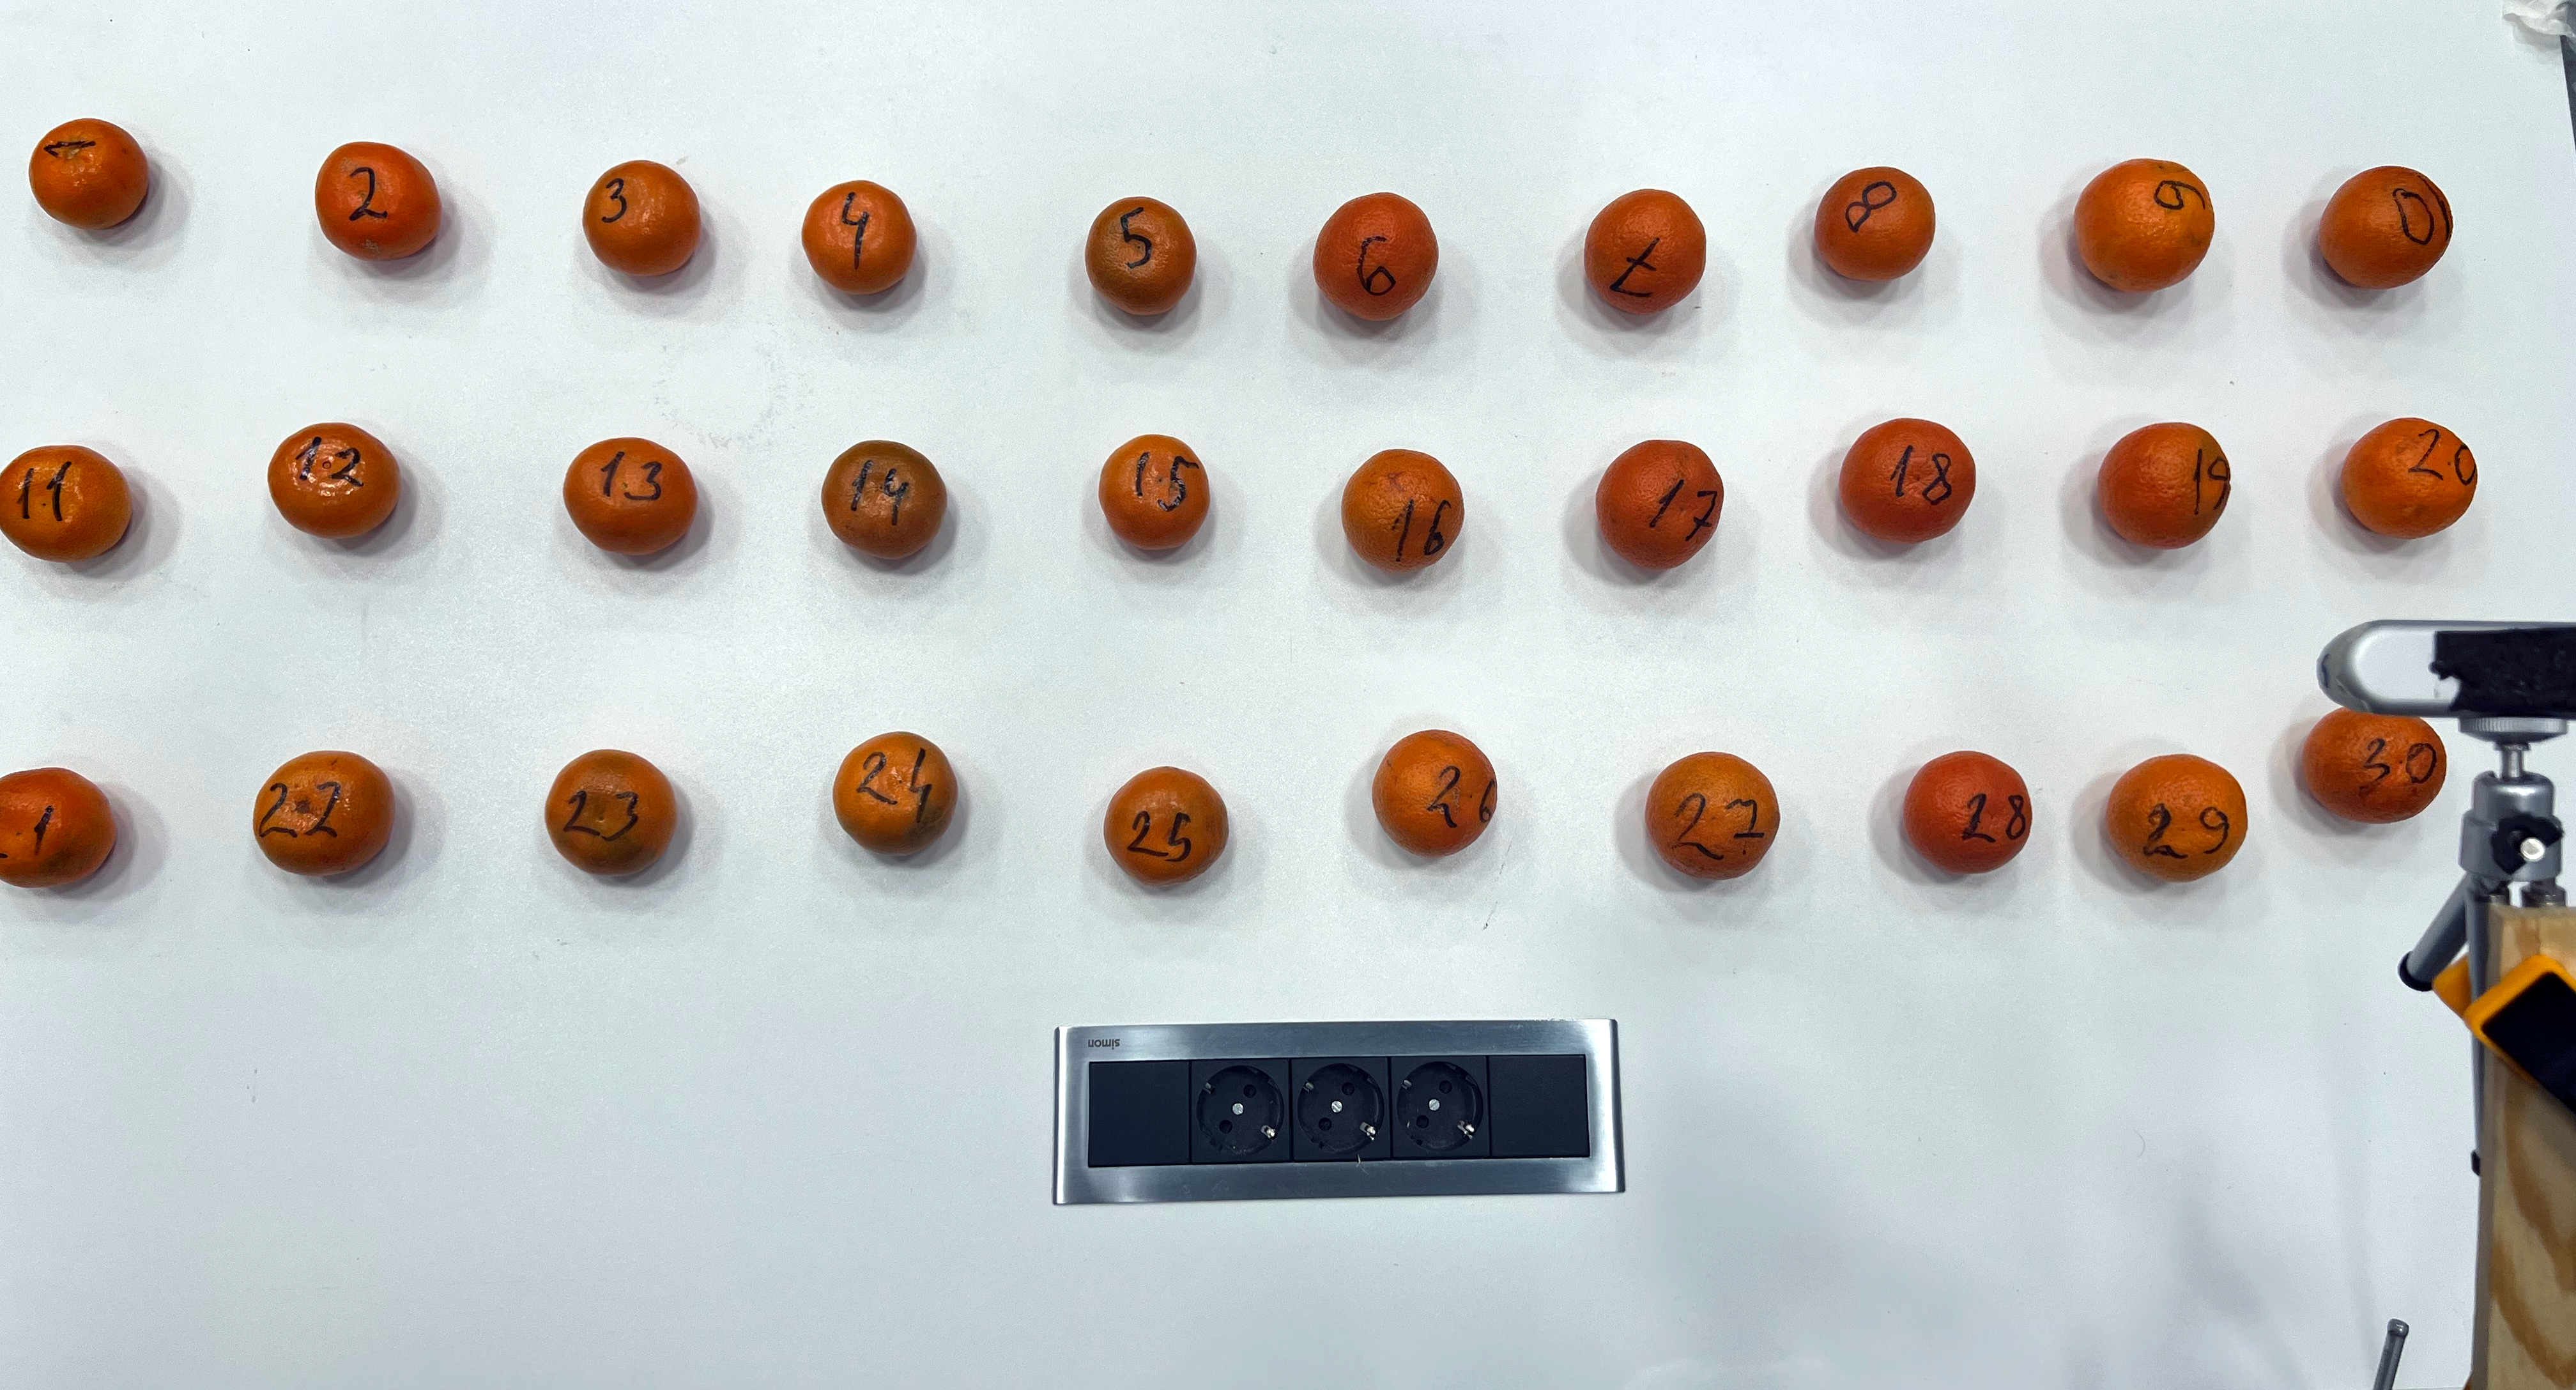
\includegraphics[width=0.8\textwidth]{images/tanj_exp.png}}
\caption{RGB frame from the dataset. It contains 30 tangerines. The images and the point clouds were captured with Intel RealSense D435i camera.}
\label{tanjes}
\end{figure}

POWDERY MILDEW DATA COLLECTION

\begin{figure}
    \centering

    \begin{subfigure}[b]{0.6\textwidth}
        \centering
        \includegraphics[width=\textwidth]{images/photo_with_disease_1_2.png}
        \caption{Image of powdery mildew-infected leaves.}
        \label{fig_photo_with_powdery_mildew}
    \end{subfigure}
    \hfill
    \begin{subfigure}[b]{0.6\textwidth}
        \centering
        \includegraphics[width=\textwidth]{images/photo_with_disease_2_2.png}
        \caption{A scattering of white patches is a clear visual sign of the presence of the disease.}
        \label{fig_photo_with_powdery_mildew_zoomed}
    \end{subfigure}
    \caption{(a) Image from the bottom camera of the robot. (b) Zoomed in.}
    \label{fig_leaves}
\end{figure}
%\ref{fig:camera_positioning}

\section{Data markup and quality evaluation}
\label{Markup}
A set of approximately 300000 images was collected with some of them exhibiting manifestations of the powdery mildew, see Figures \ref{fig_photo_with_powdery_mildew}, \ref{fig_photo_with_powdery_mildew_zoomed}.
%This figure encompasses all feasible frames extracted from individual video segments acquired through passages alongside tomato rows, utilizing three cameras.
In order to obtain a dataset of a reasonable size, every 30-th frame was chosen, resulting in approximately 10000 frames that are uniformly distributed across the entire original dataset.

%This approach was employed to introduce greater diversity in the frames, accounting for the robot's movement speed and the frames captured per second.
%Additionally, this downsampling was implemented to enhance operational efficiency by working with a subset of the dataset, rather than the entire population, thus facilitating more manageable analysis and processing.
The process of the data labeling was organized as follows.
At each of the 4 iterations, each of the experts was provided with 550 images of the tomato leaves, which had to be separated into two classes: negative and positive.
Among these 550 images, there were 500 unique for each expert and 50 images shared by all the experts in order to assess their consistency.
The mutual consistencies of the experts in the subsets are given in Table \ref{Tab:consistencies}.

\begin{table}[ht]
    %\begin{subtable}[h]{0.90\textwidth}
    \centering
    \begin{tabularx}{0.82\textwidth}{ 
        | >{\centering\arraybackslash}X 
        | >{\centering\arraybackslash}X 
        | >{\centering\arraybackslash}X 
        | >{\centering\arraybackslash}X 
        | >{\centering\arraybackslash}X | }
        \hline
    Markers & A & B & C & D  \\ \hline
    A & 1.0 & 0.72 & 0.88 & 0.82 \\ \hline
    B &     & 1.00 & \textbf{0.60} & 0.90 \\ \hline
    C &     &      & 1.00 & \textbf{0.70} \\\hline
    D &     &      &      & 1.00 \\
    \hline
    \end{tabularx}
    \caption*{1 iteration}
    
    %\label{tab:1iter}
    %\end{subtable}

    %\hfill
    %\begin{subtable}[h]{0.90\textwidth}
    \centering
    \centering
    \begin{tabularx}{0.82\textwidth}{ 
        | >{\centering\arraybackslash}X 
        | >{\centering\arraybackslash}X 
        | >{\centering\arraybackslash}X 
        | >{\centering\arraybackslash}X 
        | >{\centering\arraybackslash}X | }
        \hline
    Markers & A & B & C & D  \\ \hline
    A & 1.0 & 0.88 & \textbf{0.68} & 0.96 \\ \hline
    B &      & 1.00 & 0.80 & 0.92 \\ \hline
    C &      &      & 1.00 & 0.72 \\\hline
    D &      &      &      & 1.00 \\
    \hline
    \end{tabularx}
    \caption*{2 iteration}
    %\label{tab:2iter}
    %\end{subtable}

    %\hfill
    %\begin{subtable}[h]{0.90\textwidth}
    \centering
    \centering
    \begin{tabularx}{0.82\textwidth}{ 
        | >{\centering\arraybackslash}X 
        | >{\centering\arraybackslash}X 
        | >{\centering\arraybackslash}X 
        | >{\centering\arraybackslash}X 
        | >{\centering\arraybackslash}X | }
        \hline
    Markers & A & B & C & D  \\ \hline
    A & 1.0 & 0.92 & 0.86 & 0.90 \\ \hline
    B &      & 1.00 & 0.94 & 0.98 \\ \hline
    C &      &      & 1.00 & 0.96 \\\hline
    D &      &      &      & 1.00 \\
    \hline
    \end{tabularx}
    \caption*{3 iteration}
    %\begin{subtable}[h]{0.90\textwidth}
    \centering
    \centering
    \begin{tabularx}{0.82\textwidth}{ 
        | >{\centering\arraybackslash}X 
        | >{\centering\arraybackslash}X 
        | >{\centering\arraybackslash}X 
        | >{\centering\arraybackslash}X 
        | >{\centering\arraybackslash}X | }

        \hline
    Markers & A & B & C & D  \\ \hline
    A & 1.0 & 0.94 & 0.92 & 0.92 \\ \hline
    B &      & 1.00 & 0.89 & 0.86 \\ \hline
    C &      &      & 1.00 & 0.92 \\\hline
    D &      &      &      & 1.00 \\
    \hline
    
    \end{tabularx}
    \caption*{4 iteration}
    %\caption{\label{Tab:consistencies} Each subtable represents one of 4 iterations of the data markup. A, B, C, and D in the tables represent the individual human experts. The number in $ij$-th element of the table represents the share of the matching labels (positive or negative) for the corresponding experts on a subset of 50 images that they shared during that iteration.}
    \caption{\label{Tab:consistencies} Tables of mutual consistencies of the human experts.} Each table represents one of 4 iterations of the data markup. The consistencies of $0.7$ and below are highlighted in bold. A, B, C, and D in the tables represent individual human experts. The number in $ij$-th element of the table is the fraction of the matching labels (positive or negative) for the corresponding experts on a subset of 50 images that they shared during that iteration. The mean consistency (excluding the consistency of the experts with themselves) is $0.8579$, which closely matches the accuracy of the best model.
\end{table}

It is worth noting, that the major part of inconsistencies occur as a consequence of the frame quality. It is possible to overcome this issue by reducing motion blur with the help of the cameras with a global shutter, however, this work shows that the target problem can be solved with cameras with a rolling shutter.

\section{Data}
\label{sec:data}

\subsection{Experimental setup}
\label{subsec:setup}

The view of the stand is given in Figure~\ref{fig:algo_nn}.

The dataset was collected by simulating the static scenario of the robotic platform aquiring the data while being positioned on the pipe rails.
The RealSense D435i camera was mounted vertically downward at a height of 0.9 \si{m} from the base of the rails.
To capture the lower row of plants, a branch was hang with tomatoes 0.80 \si{m} away from the camera, ensuring all fruits were in sight.
This setup positioned the tomatoes between 0.92 \si{m} and 1.27 \si{m} from the camera lens, with a horizontal spread of approximately 0.2 \si{m}.

The data was recorded data using both RGB and Depth channels, synchronized via standard RealSense SDK methods.
Each tomato was physically marked for identification during post-processing.
The lighting conditions were consistent, as the room was equipped with a window that blocks infrared light, and the overcast weather prevented direct sunlight.

By default, auto-exposure and auto-white balance settings were used, which were stable enough for short captures, as confirmed by minimal hyperparameter changes in the frame metadata. The resolution was set to 1920$\times$1080 for RGB and 1280$\times$720 for depth at 30 FPS.

The Fields of View of the cameras are the following.
\begin{itemize}
    \item Depth FOV: $87^\circ \times 58^\circ$
    \item RGB FOV: $69^\circ \times 42^\circ$
\end{itemize}

Given the platform's maximum speed of 1.5 \si{m/s}, an evaluation was carried out in order to assure that the rate of 30 FPS was sufficient to avoid motion blur.

\subsection{Data description and storage}
\label{subsec:data_storage}

All the data consists of two parts: synthetic and real.
Regarding the synthetic data, full ellipsoids were considered, segments of ellipsoids, noisy full ellipsoids and noisy ellipsoid segments.

Regarding the real data, after the point clouds are cropped by YOLO, all the cropped raw points alongside the ground truth data are stored in numpy $.npz$ format.
The number of point clouds is the following:
\begin{itemize}
    \item 146 point clouds with 14 tomatoes each for the real data
    \item 200 point clouds for clean data
    \item 200 for clean segment
    \item 900 for noised full ellipsoids
    \item 1100 for segments of noised segments
\end{itemize}

In order to obtain the ellipsoid model, and .npz file is loaded, and 1000 for synthetics and 1000 for polygon sets of 9 points are sampled from the point cloud  with permutations and without replacement to ensure no duplicate sets exist using torch library to speed up the process using GPU.
For each 10000 iteration a system of equations is formed and solved.
The results are stored in their entirety using numpy .npz format.

For each combination of hyperparameters (43 for polygon and 67 for synthetics), a table with 1000 rows and 52 columns, including the predicted characteristics and IoU, is produced.
It is stored as a columnar data in parquet files for the sake of low storage capacity to overcome and reduce the potential capacity requirement down to almost 100 GB overall.

Analysing all data at once would become difficult considering 100 GB of data and only 16 GB of RAM capacity.
Thus, DuckDB database system supporting parquet format and SQL queries is used.
In order to ease the analysis, each time a filter predicate is defined and a SQL query executed through DuckDB to benefit from both the high read/write speed and low memory usage. The data received from DuckDB, then is stored in a polars dataframe as a tool for analysis. 
